\section{Ablauf}
\section*{Steuerelemente des Bad-Designers}
\begin{figure}[h]
    \centering
    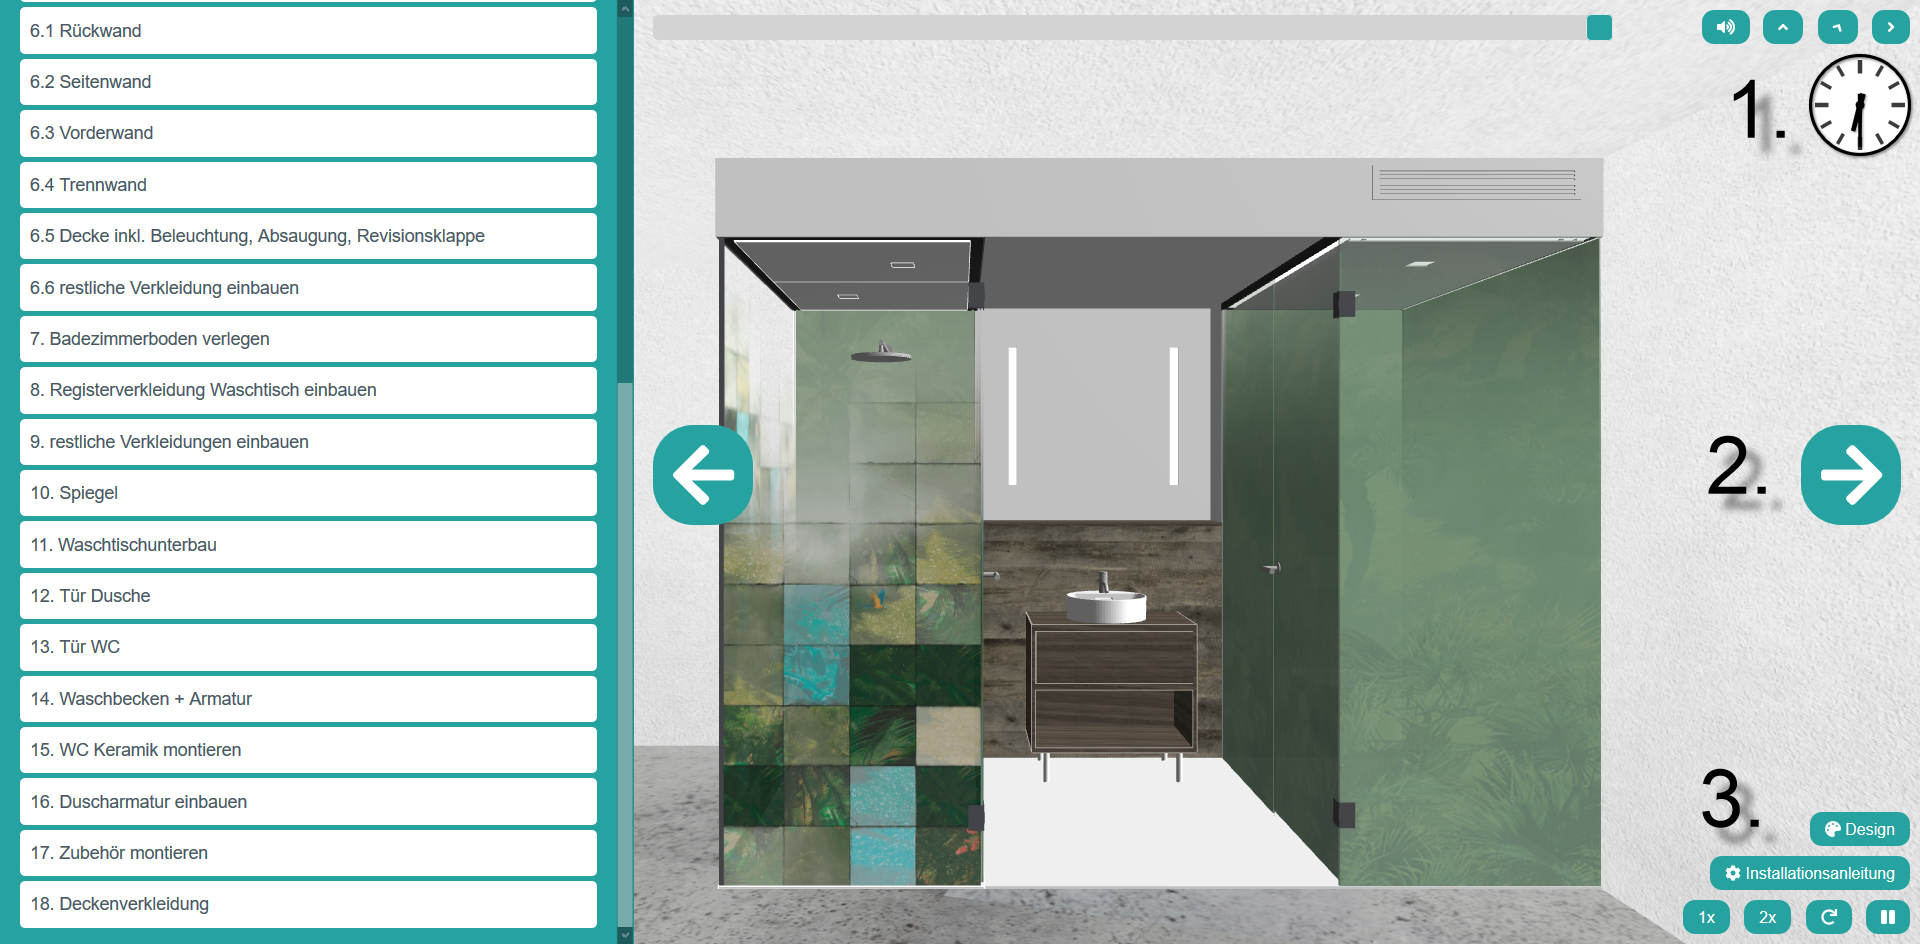
\includegraphics[width=1\linewidth]{images/screenshots/00_button_desc.png}
    \caption{Steuerelemente des Bad-Designers}
    \label{}
\end{figure}
\noindent In der ersten Gruppe der Steuerelemente befinden sich vier Buttons und eine Uhr. Der erste Button schaltet die Hintergrundmusik auf Stumm, die anderen drei dienen zum einstellen der Perspektive. Insgesamt gibt es drei Ansichten, nämlich die Frontansicht, die Schrägansicht und die Seitenansicht. Die darunter befindliche Uhr zeigt an wie viel Zeit der Einbau des jeweiligen Bauteiles veranschlagt.\\
Die zweite Gruppe steuert die Designs der Bäder, mit den großzügigen Pfeilen kann man mühelos sich alle Designs zum selben Grundriss ansehen.
\\
Die dritte Gruppe dient zur Steuerung der Animationen. Man kann dabei die Animationsgeschwindigkeit einstellen, die Installationsanleitung neu starten oder pausieren. Mit den Buttons \dq Design\dq und \dq Installationsanleitung\dq steuert man die Liste am linken Bildschirmrand, also sie zeigt dann dementsprechend die Designs oder die einzelnen Schritte der Installationsanleitung.
\clearpage \newpage
\begin{figure}[h]
    \centering
    
\includegraphics[width=1\linewidth]{images/screenshots/00.png}
    \caption{Ladeseite vom Bad-Designer}
    \label{}
\end{figure}
\noindent Auf diesem Bild ist die Ladeseite des Bad-Designers zu sehen. Während im Hintergrund bereits die Bäder geladen werden sieht man den Fortschritt an der Ladeanimation am unteren Bildschirmrand.



\begin{figure}[h]
    \centering
    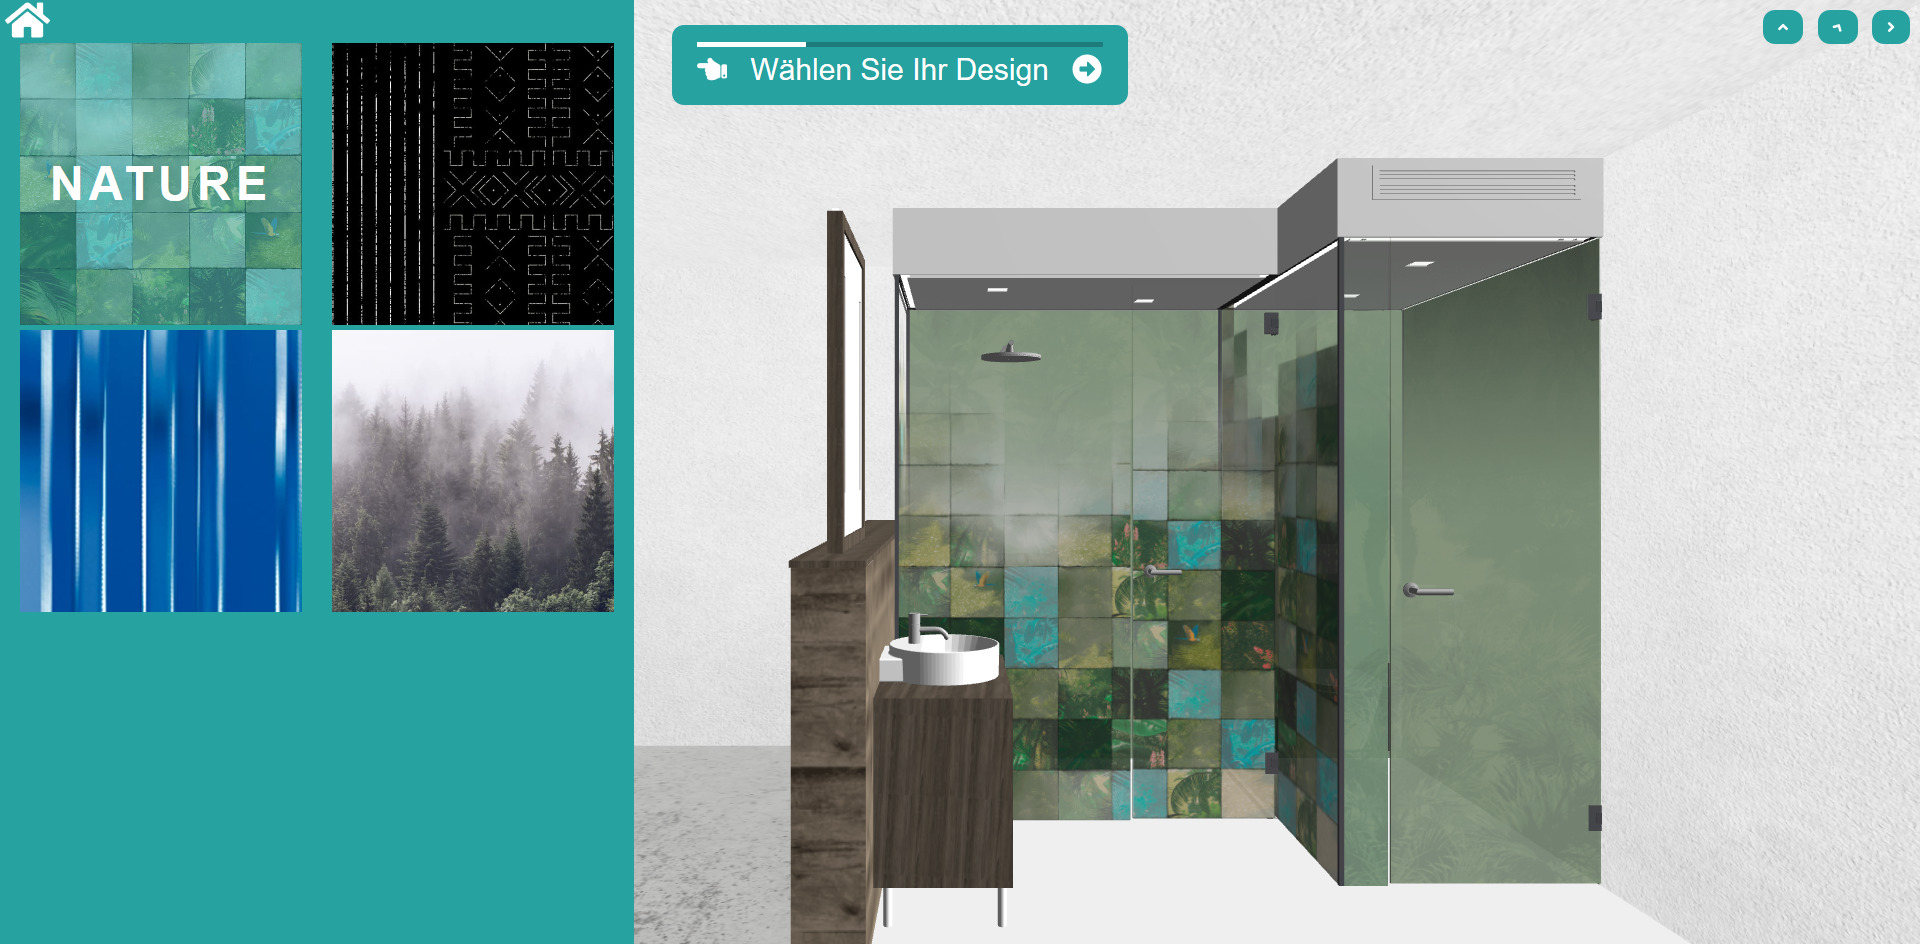
\includegraphics[width=1\linewidth]{images/screenshots/01.png}
    \caption{Startseite vom Bad-Designer}
    \label{}
\end{figure}
\noindent Auf diesem Bild ist die Startseite des Bad-Designers zu sehen. Es wird sofort ein fertiges Badezimmer angezeigt mit einem vorgewähltem Design. Jedoch kann man sich hier noch für ein anderes Design umentscheiden, anschließend kann man per Mausklick auf den rechten Pfeil oder nach ein paar Sekunden automatisch zur Grundrissauswahl gehen.
\clearpage \newpage
\begin{figure}[h]
    \centering
    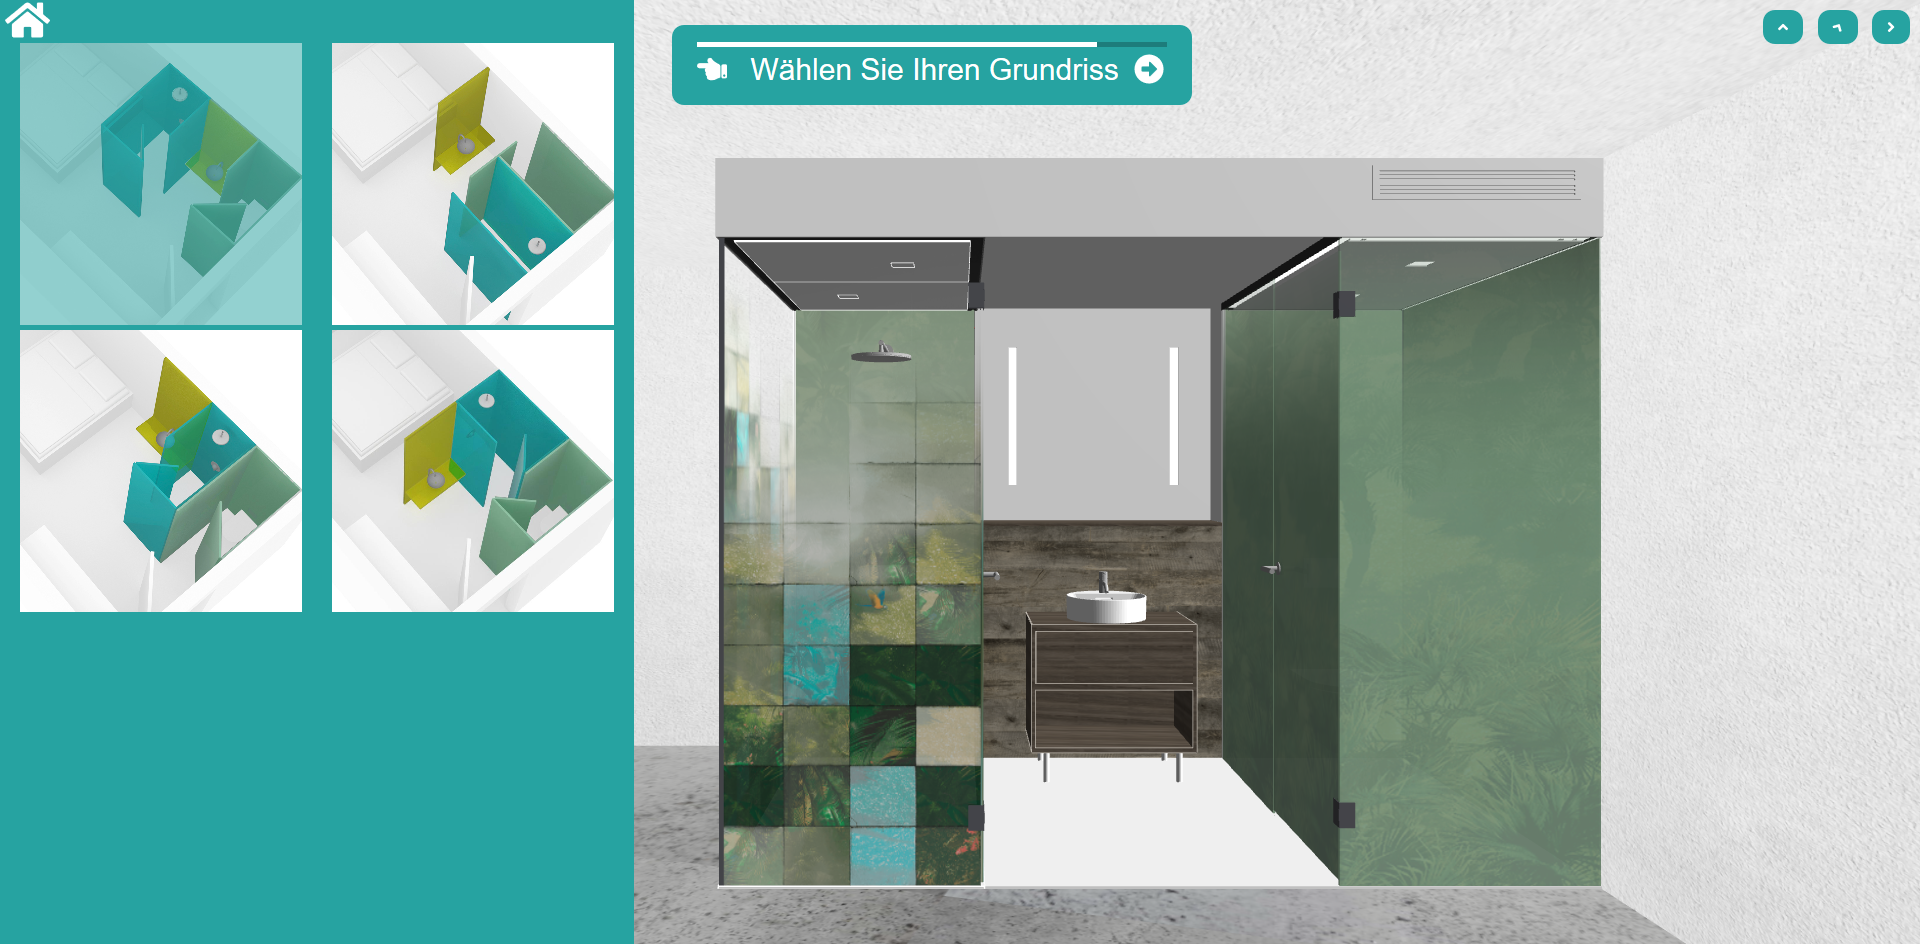
\includegraphics[width=1\linewidth]{images/screenshots/02.png}
    \caption{Grundrissauswahl}
    \label{}
\end{figure}
\noindent Als nächstes wird der Benutzer vor die Wahl gestellt, welchen Grundriss er sehen und bauen lassen will. Für die weitere Anleitung wurde der erste Grundriss ausgewählt.

\begin{figure}[h]
    \centering
    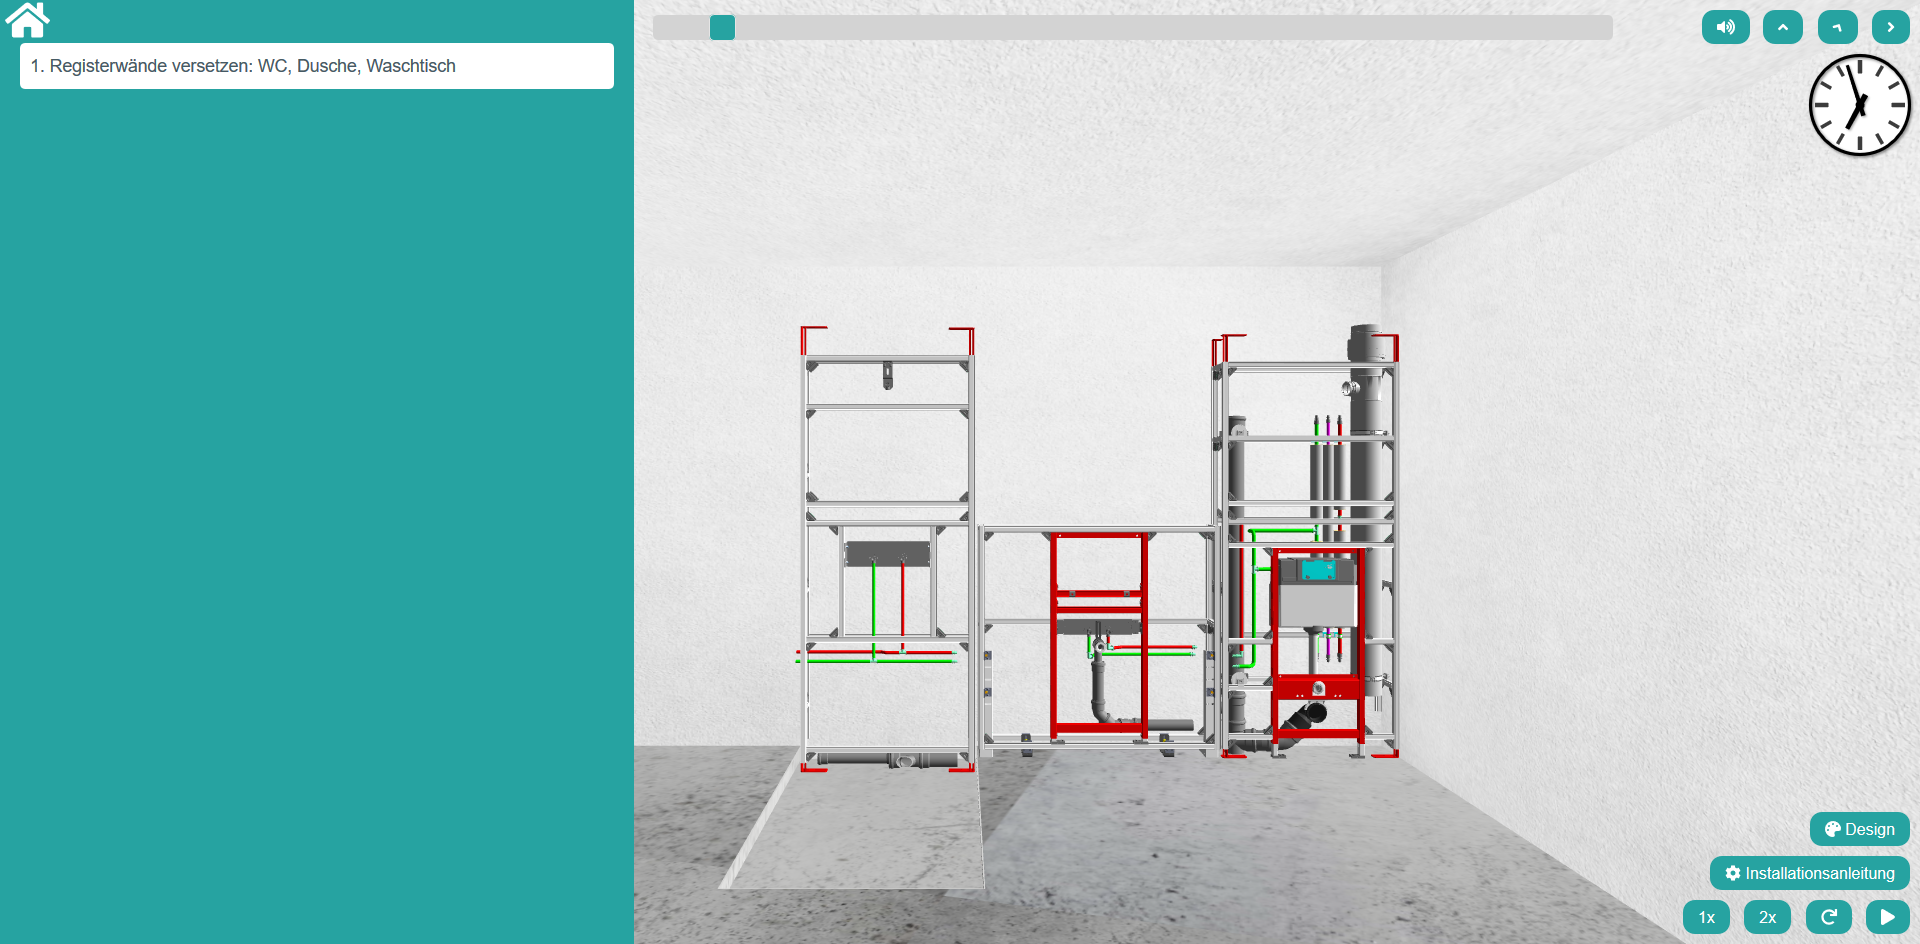
\includegraphics[width=1\linewidth]{images/screenshots/03.png}
    \caption{Einbau der Register}
    \label{}
\end{figure}
\noindent Wenn man sich für die Installationsanleitung entschieden hat, werden als erstes die Register eingebaut.

\clearpage \newpage

\section*{Detailansichten}
\begin{figure}[h]
    \centering
    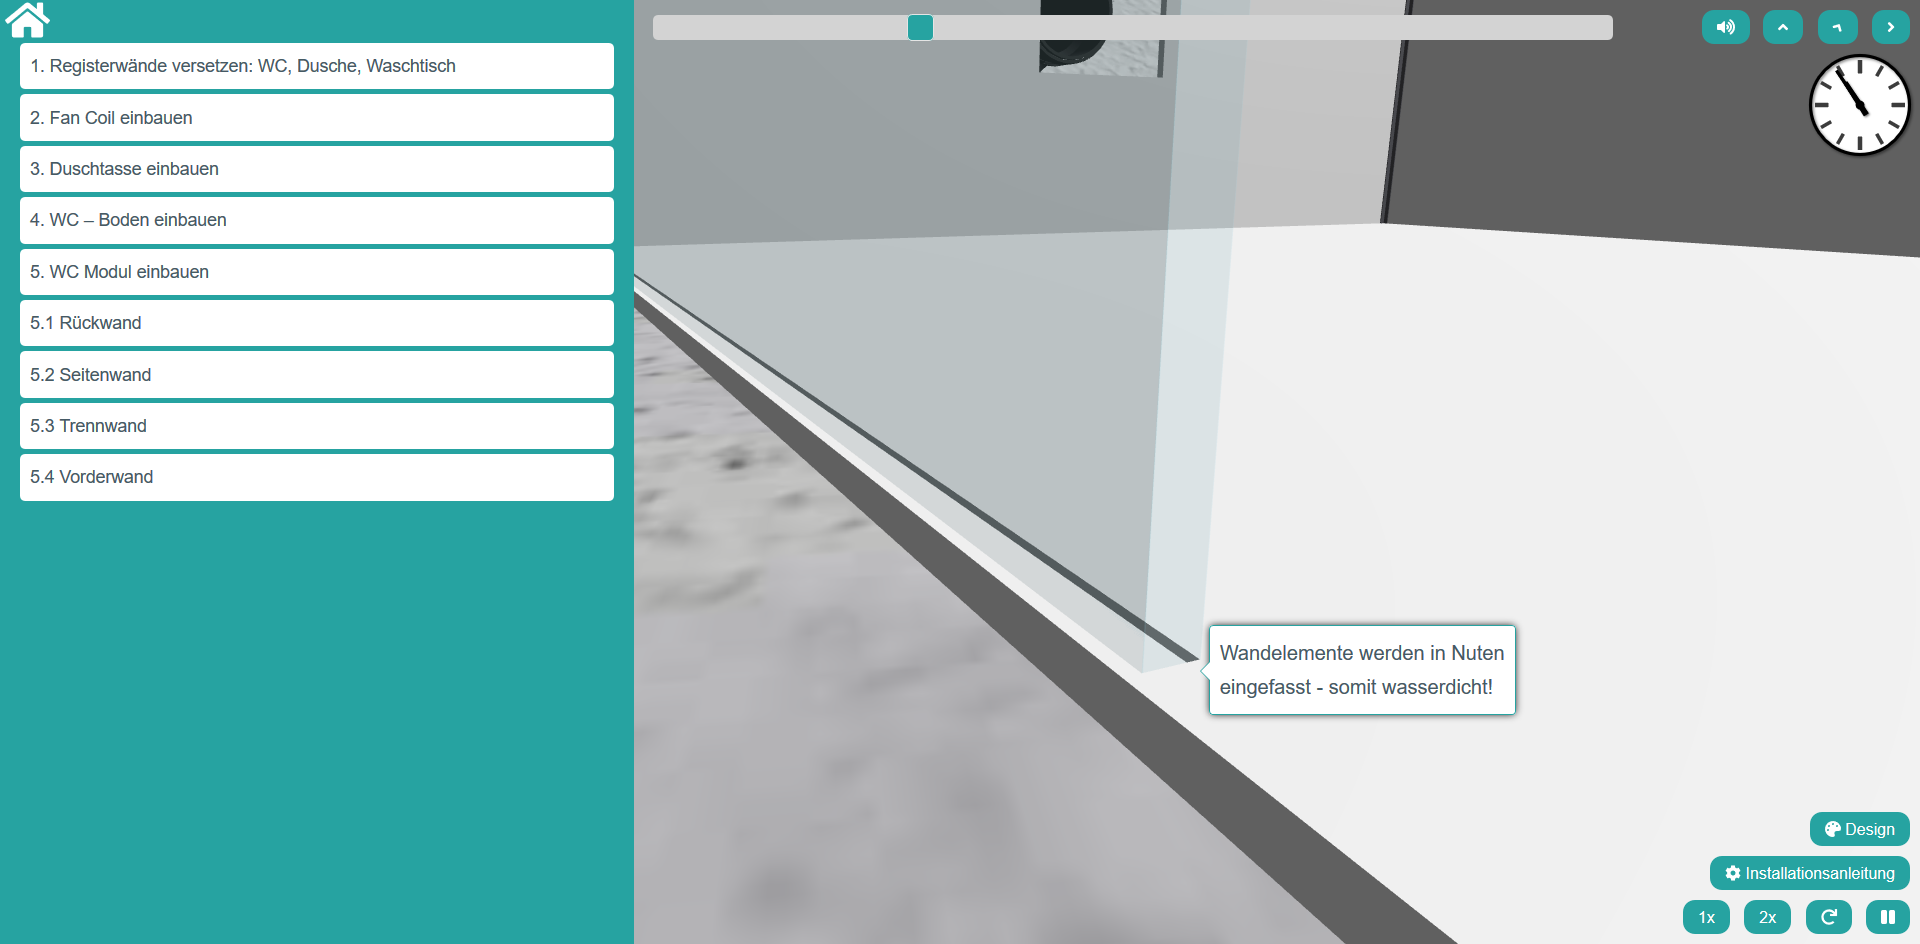
\includegraphics[width=1\linewidth]{images/screenshots/04.png}
    \caption{Detailansicht der Wandelemente}
    \label{}
\end{figure}
\noindent Im Laufe der Installation erscheinen Detailansichten, die die Besonderheiten der SanMOD Bäder hervorheben. 



\begin{figure}[h]
    \centering
    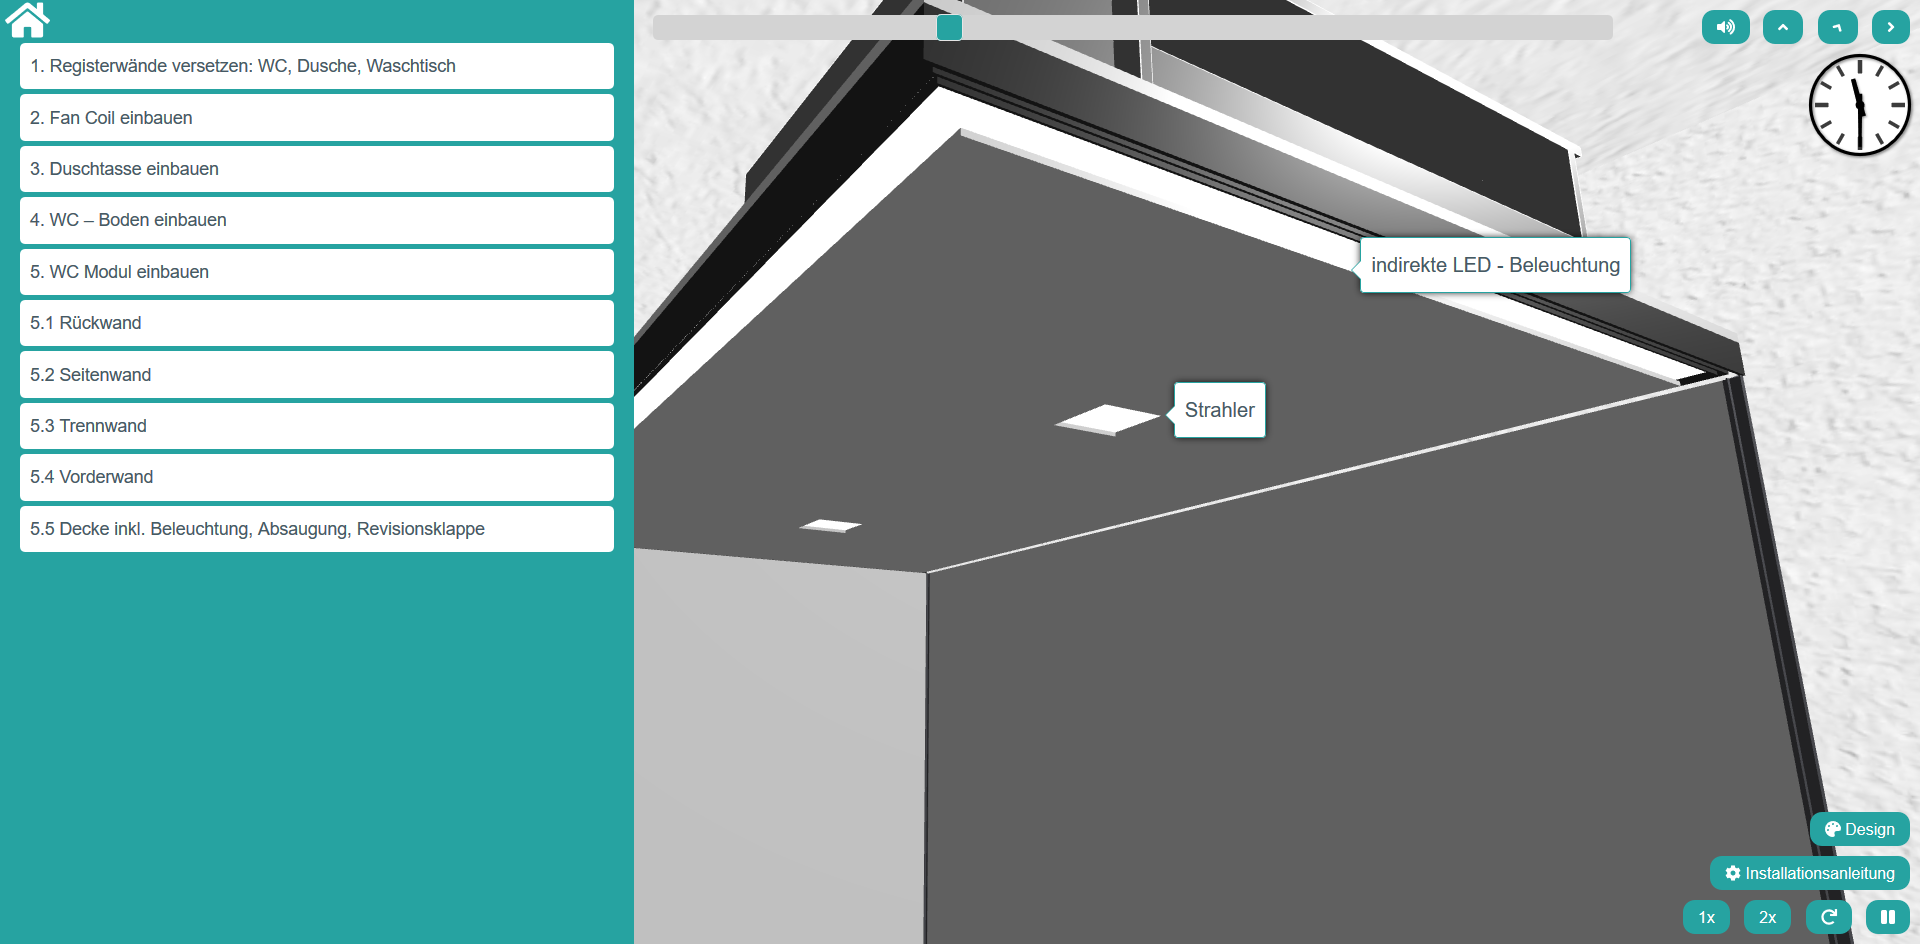
\includegraphics[width=1\linewidth]{images/screenshots/05.png}
    \caption{Detailansicht: Deckenbeleuchtung}
    \label{}
\end{figure}
\noindent Diese Detailansicht stellt die Deckenbeleuchtung in der Dusche dar.
\clearpage \newpage
\begin{figure}[h]
    \centering
    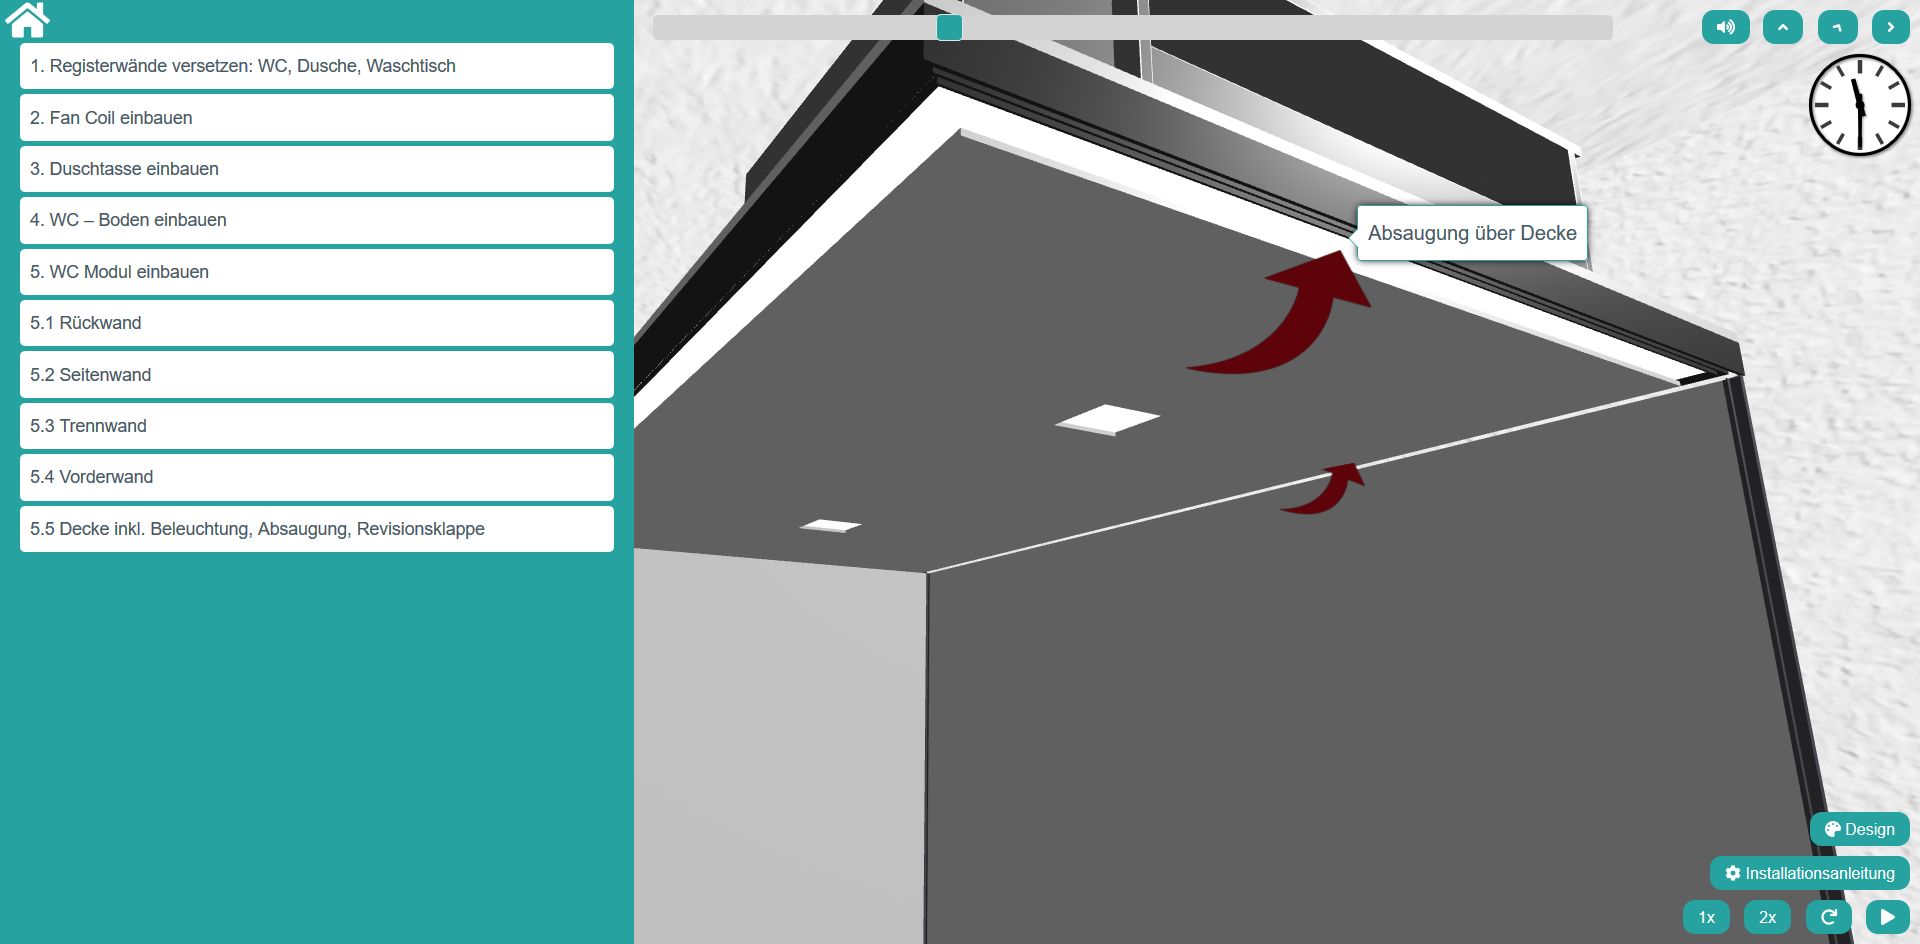
\includegraphics[width=1\linewidth]{images/screenshots/06.png}
    \caption{Detailansicht: Dampfabzug}
    \label{}
\end{figure}
\noindent Hier wird der Dampfabzug in der Dusche im Detail angezeigt.



\begin{figure}[h]
    \centering
    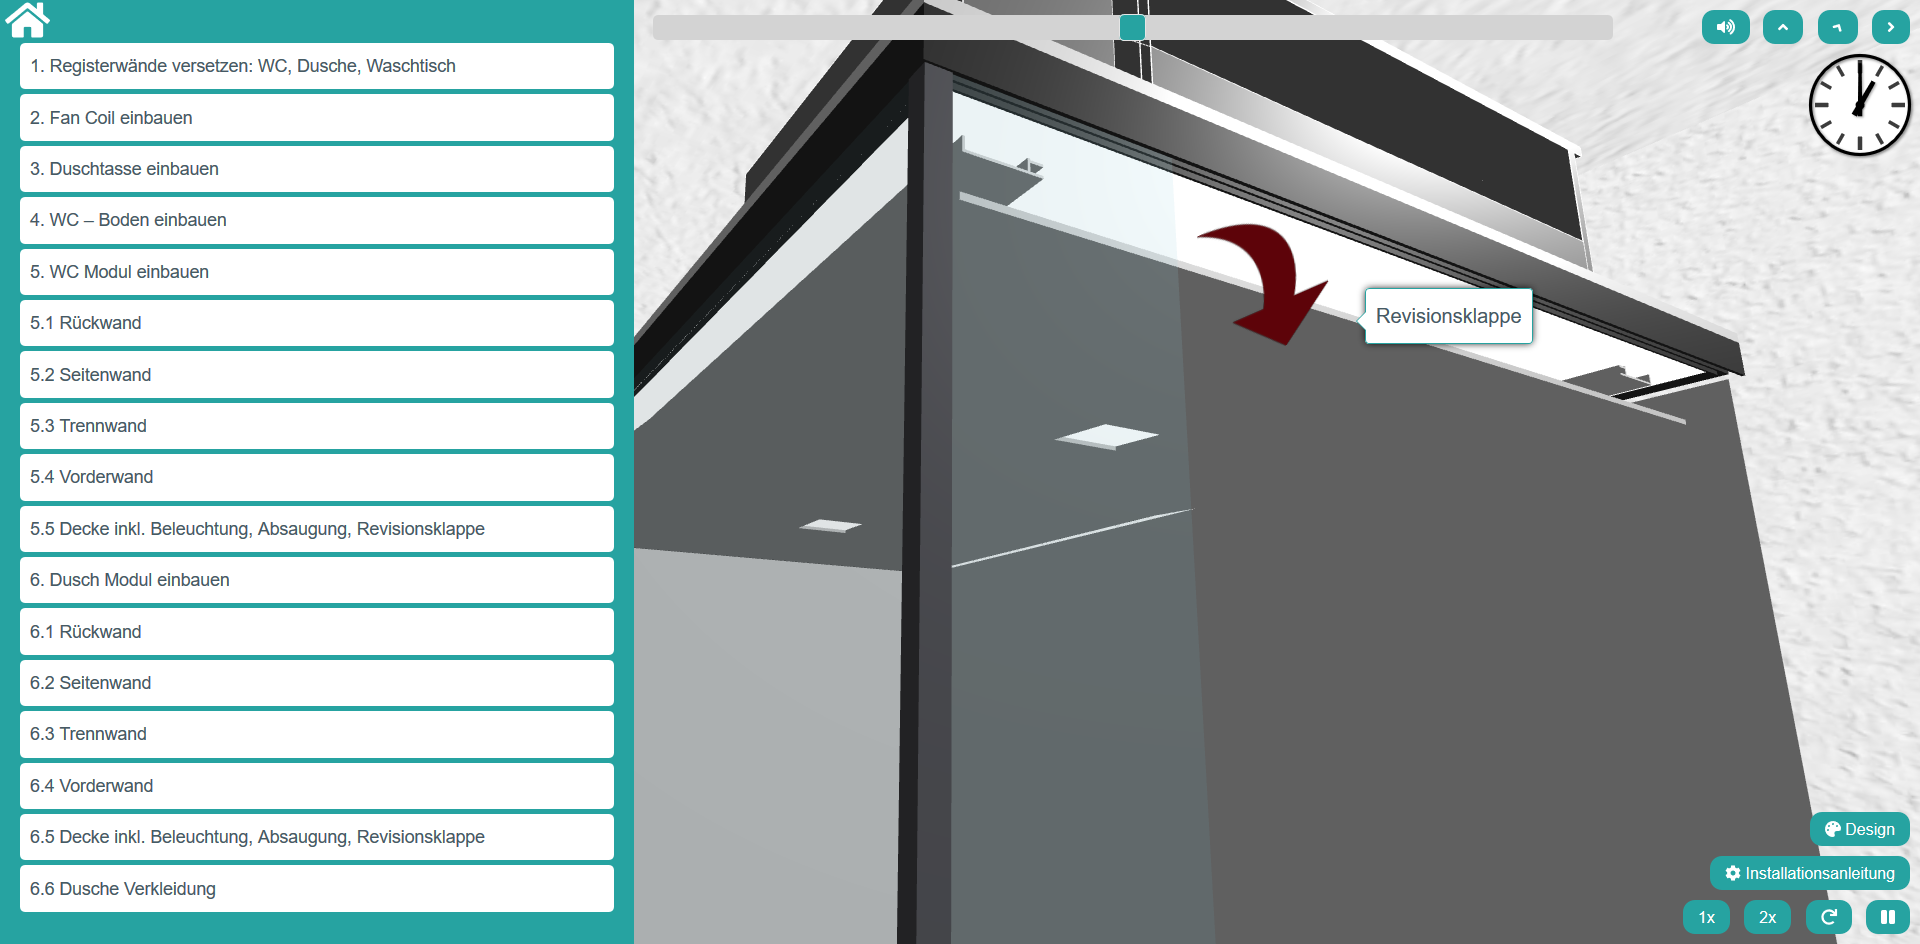
\includegraphics[width=1\linewidth]{images/screenshots/06a.png}
    \caption{Detailansicht: Revisionsklappe}
    \label{}
\end{figure}
\noindent Die Revisionsklappe ermöglicht es ohne größeren Aufwand an das Innenleben heranzukommen.
\clearpage \newpage
\begin{figure}[h]
    \centering
    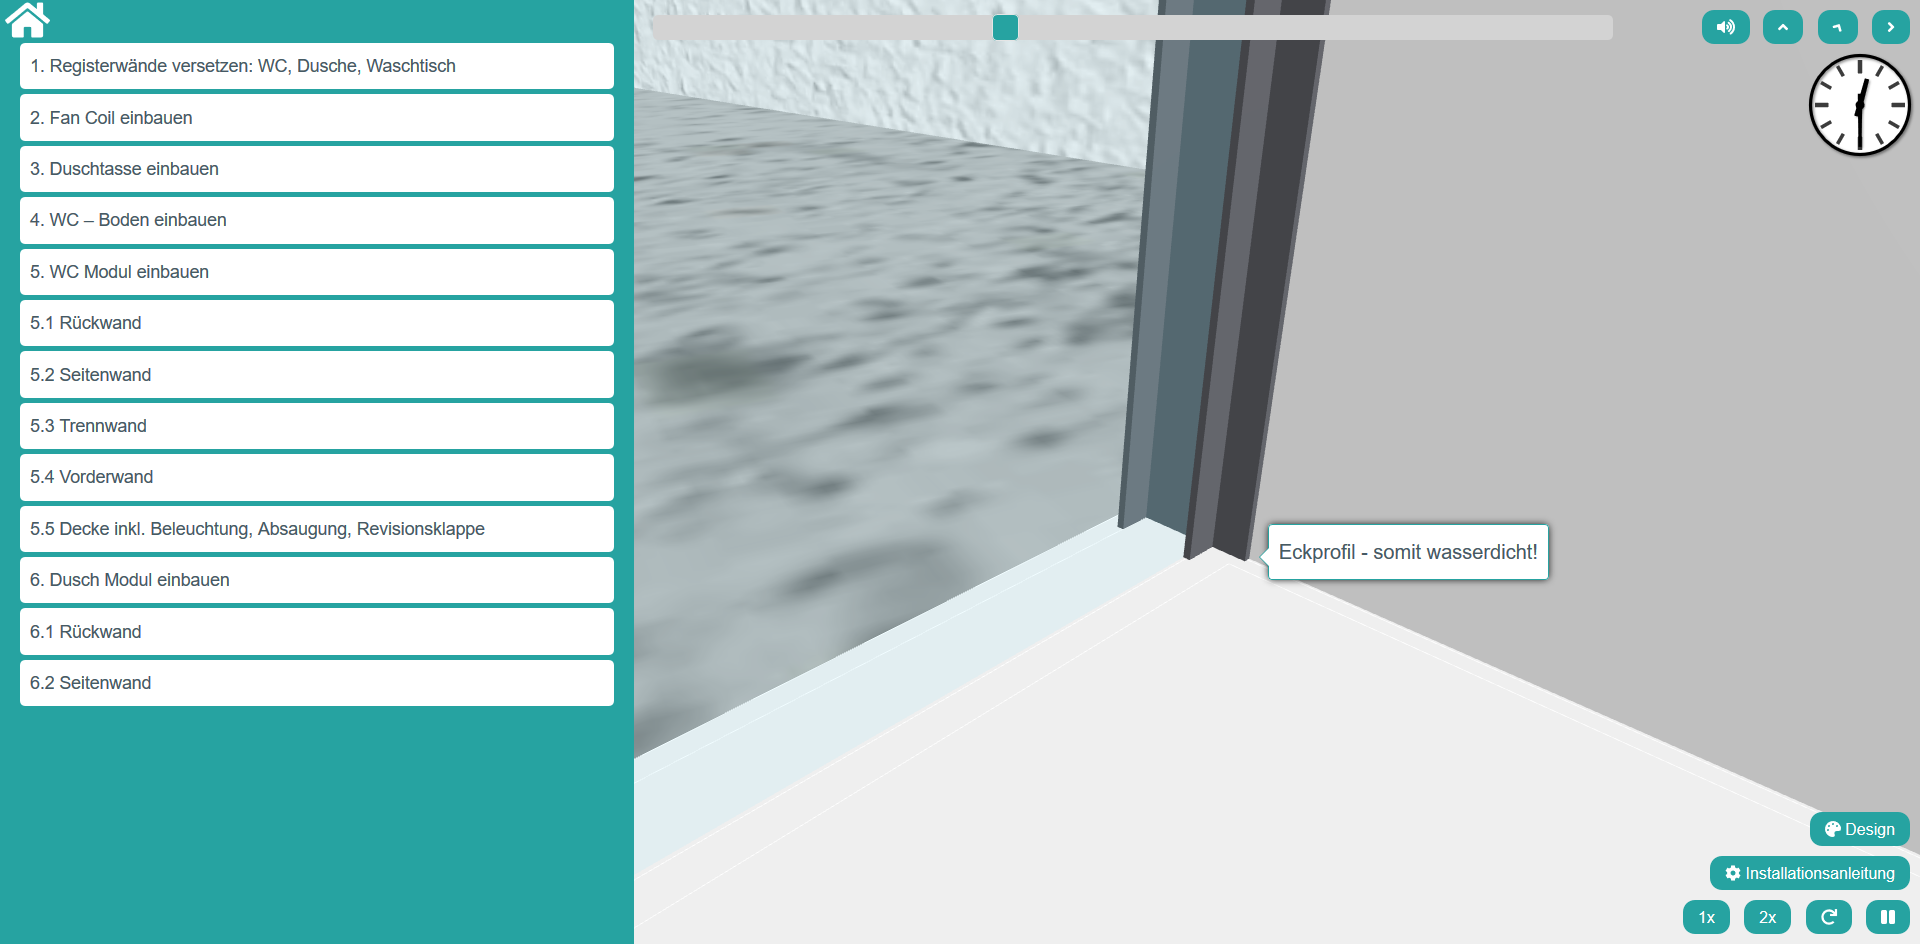
\includegraphics[width=1\linewidth]{images/screenshots/07.png}
    \caption{Detailansicht: Eckprofil}
    \label{}
\end{figure}
\noindent Das Eckprofil ist in einer Schiene eingefasst und somit wasserdicht.

\begin{figure}[h]
    \centering
    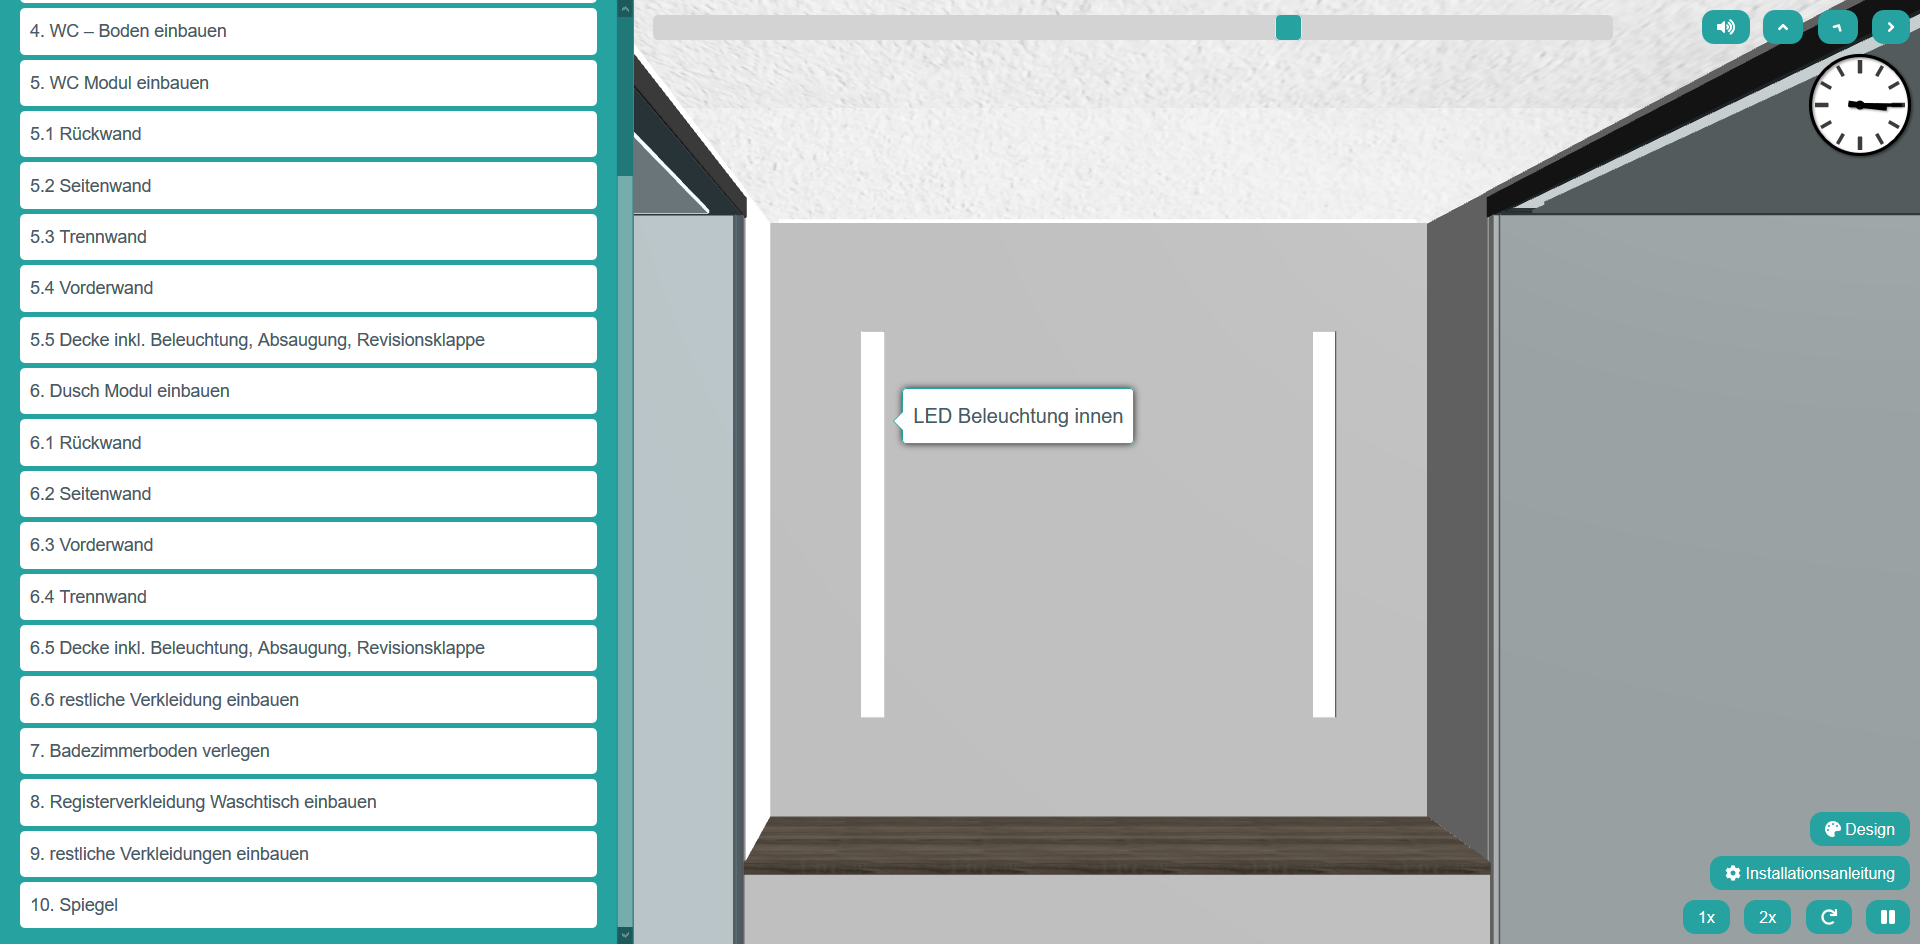
\includegraphics[width=1\linewidth]{images/screenshots/08.png}
    \caption{Detailansicht: beleuchteter Spiegel}
    \label{}
\end{figure}
\noindent Jedes Waschtischmodul [\ref{sec:waschtischmodul}] beinhaltet einen beleuchteten Spiegel.

\clearpage \newpage
\begin{figure}[h]
    \centering
    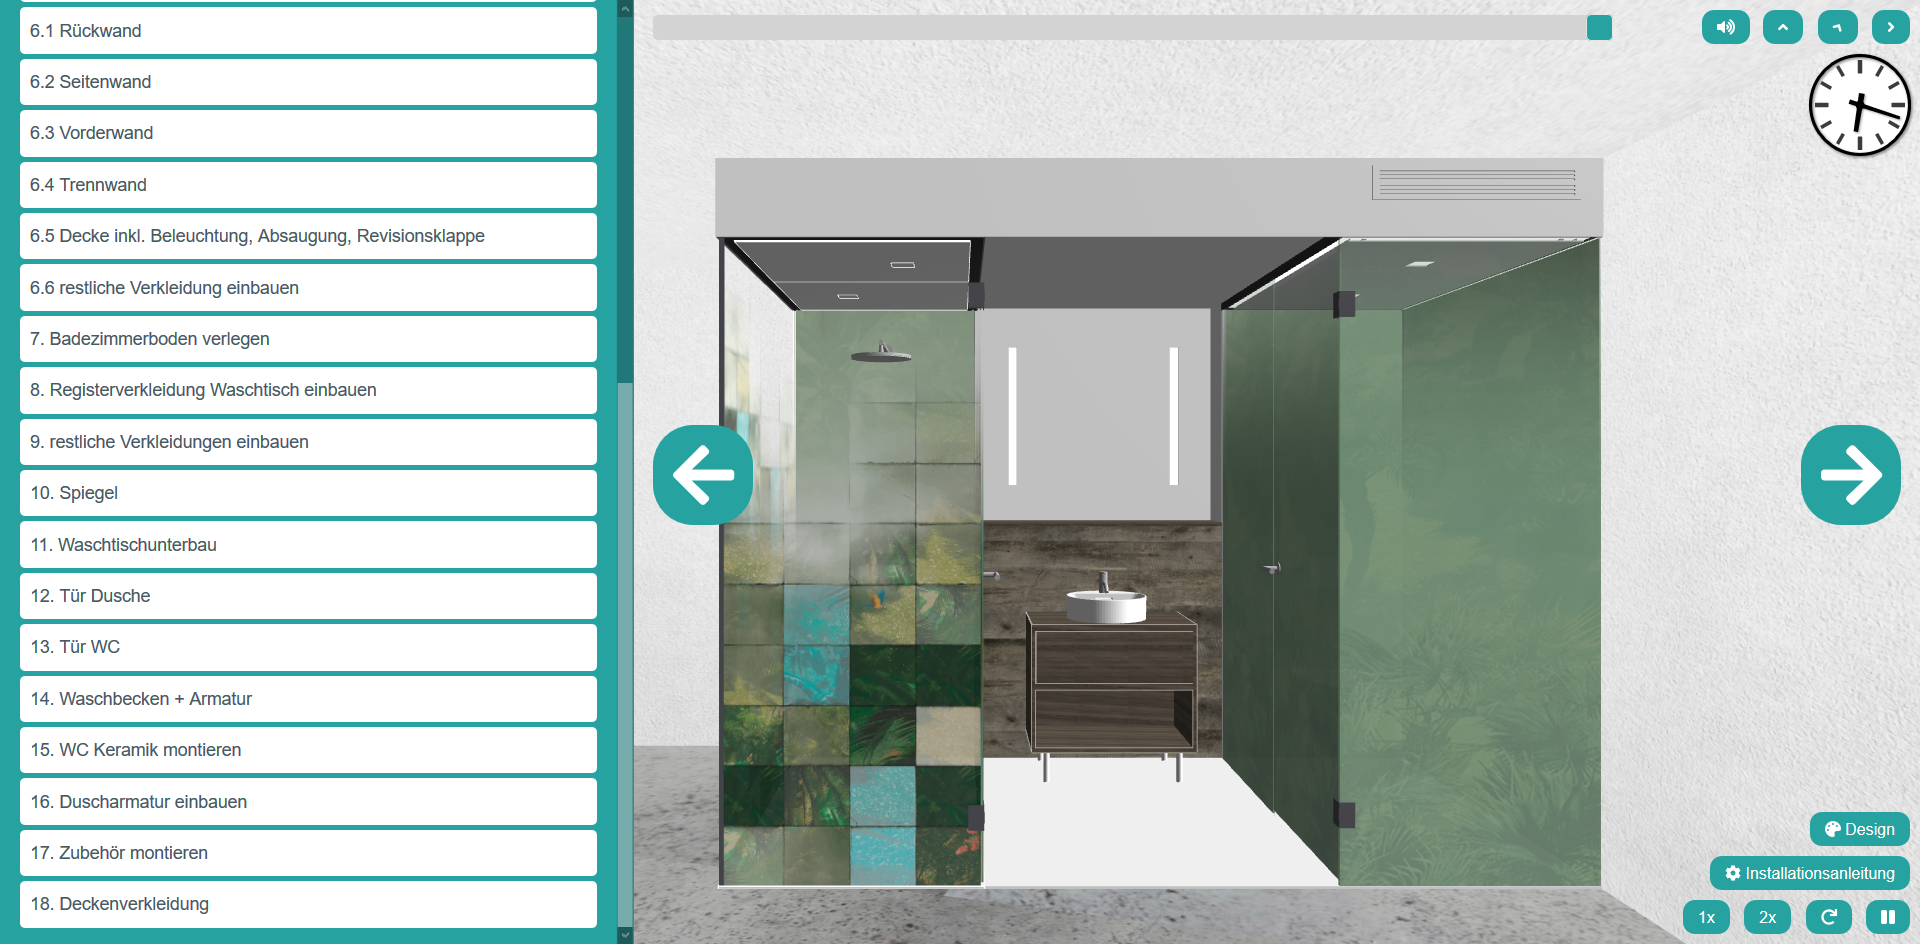
\includegraphics[width=1\linewidth]{images/screenshots/09.png}
    \caption{Fertiges Bad}
    \label{}
\end{figure}
\noindent Die Installationsanleitung ist nun zu Ende. Das fertige Bad kann aus verschiedenen Perspektiven betrachtet werden und über den Button \dq Design\dq mit einer Textur versehen werden. Mit den Pfeilen die nach rechts beziehungsweise links deuten können die Design mühelos gewecheselt werden um ein besseres Gefühl zu bekommen wie das Bad mit dem selben Grundriss mit einer anderen Textur aussieht.

\clearpage \newpage

\section*{Designauswahl}
\begin{figure}[h]
    \centering
    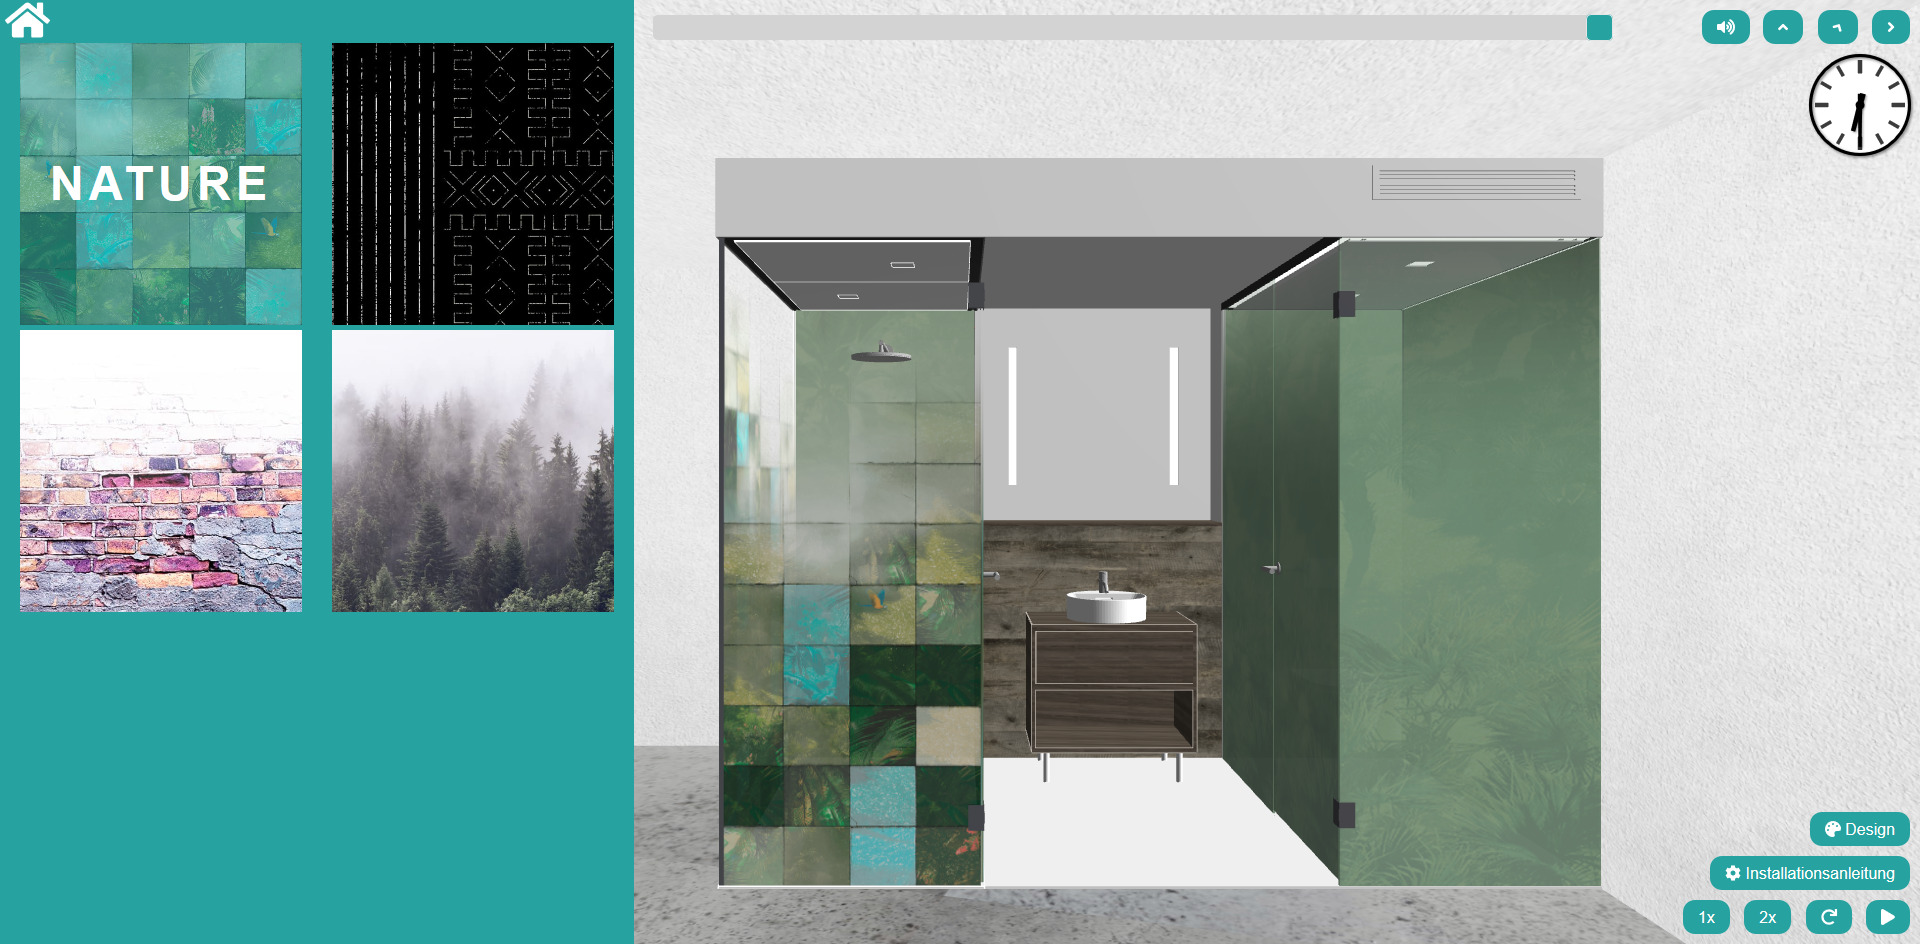
\includegraphics[width=1\linewidth]{images/screenshots/10.jpg}
    \caption{Frontansicht mit \dq Nature\dq Design}
    \label{}
\end{figure}
\noindent Auf diesem Screenshot ist das fertige Bad in der Frontansicht im \dq Nature\dq Design.

\begin{figure}[h]
    \centering
    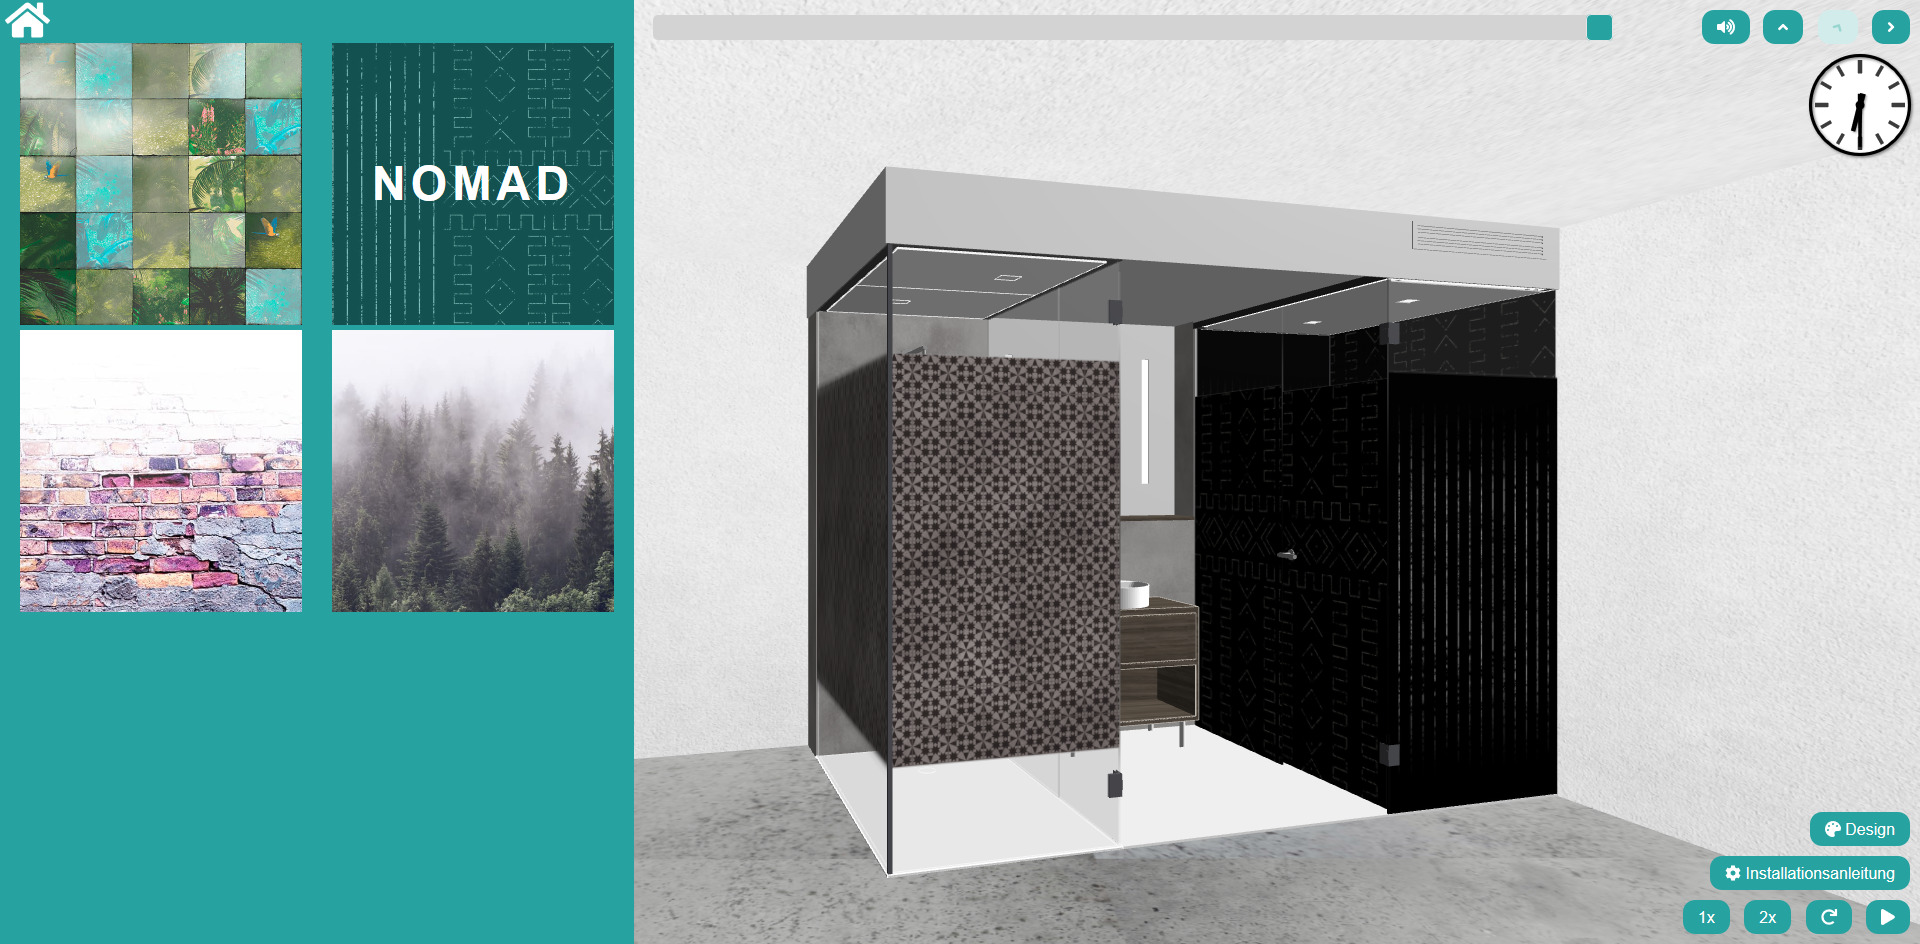
\includegraphics[width=1\linewidth]{images/screenshots/11.jpg}
    \caption{Schrägansicht mit \dq Nomad\dq Design}
    \label{}
\end{figure}
\noindent Auf diesem Screenshot ist das fertige Bad in der Schrägansicht im \dq Nomad\dq Design.